\documentclass[class=report, crop=false, 12pt,a4paper, tikz, border=4mm]{standalone}
\usepackage{enumitem}
\usepackage{float}
\usepackage{amsmath}
\usepackage{amssymb}
\usepackage[normalem]{ulem}
\usepackage{graphicx}
\usepackage{commath}
\usepackage{siunitx}
\usepackage{tikz}
\usetikzlibrary{positioning, fit, calc}   
\tikzset{block/.style={draw, thick, text width=3cm ,minimum height=1.3cm, align=center},   
line/.style={-latex}     
}
\newcommand{\Lagr}{\mathcal{L}}
\begin{document}
Previously, we have considered systems in the general sense, with a generic function block approach.
\begin{figure}[H]
  \centering
  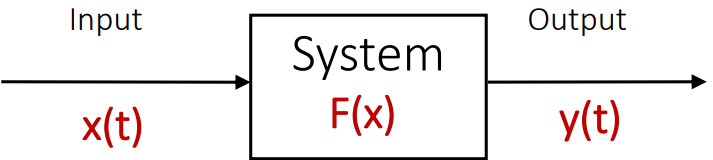
\includegraphics[width = 0.8\textwidth]{../img/blockdiagram5.png}
\end{figure}
Now we will investigate how we model physical systems and obtain the function block $F(x)$ for electrical and mechanical components.
\section{Linear Term Invariant (LTI) systems}
The focus of this course and indeed much of control theory itself focuses on modelling physical systems as \textbf{linear} and \textbf{time invariant}. LTI systems have three key properties:
\begin{itemize}
  \item Obey principle of superposition
  \item Homogeneity
  \item Time invariance
\end{itemize}
\subsection{Superposition}
If input $x_1(t)$ produces output $y_1(t)$ and input $x_2(t)$ produces $y_2(t)$, then input $x_1(t) + x_2(t)$ produces output $y_1(t) + y_2(t)$
\begin{figure}[H]
  \centering
  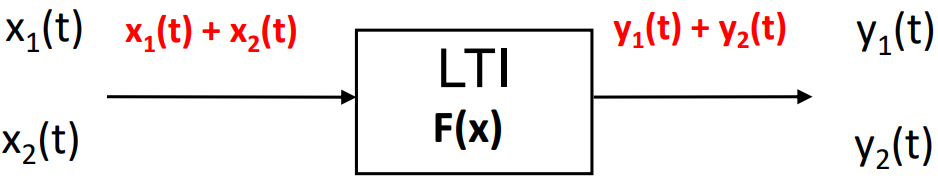
\includegraphics[width = 0.8\textwidth]{../img/blockdiagram6.png}
\end{figure}
Say for a system which doubles the input $F(x) = 2x$
\begin{figure}[H]
  \centering
  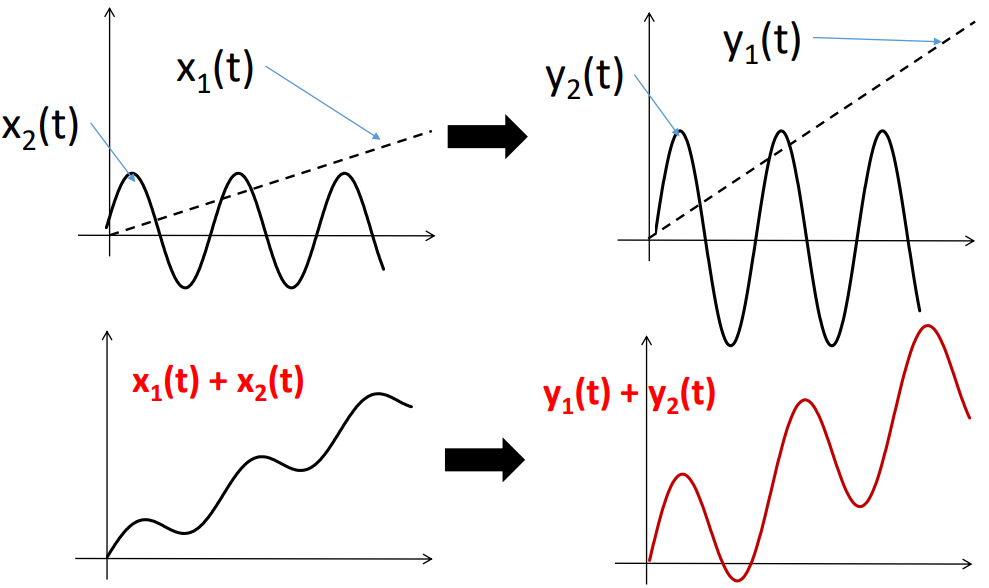
\includegraphics[width = 0.8\textwidth]{../img/graphs1.png}
\end{figure}
\subsection{Homogeneity}
If the input to the system $x(t)$ is scaled by a magnitude scale factor $A$, then the output $y(t)$ is also scaled by the same factor.
\begin{figure}[H]
  \centering
  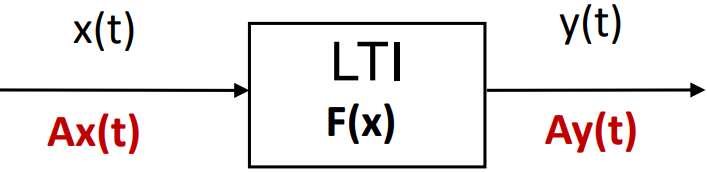
\includegraphics[width = 0.8\textwidth]{../img/blockdiagram7.png}
\end{figure}
For example, consider a system which generates a sine wave at a given amplitude, with a set frequency:
\begin{figure}[H]
  \centering
  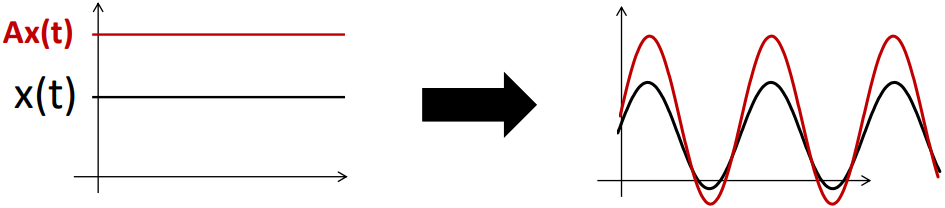
\includegraphics[width = 0.8\textwidth]{../img/graphs2.png}
\end{figure}
\subsection{Time invariance}
If input is applied at time $t=0$ or $T \ \si{\second}$ from now, the output is identical with the exception of a delay of $T \ \si{\second}$.
\begin{figure}[H]
  \centering
  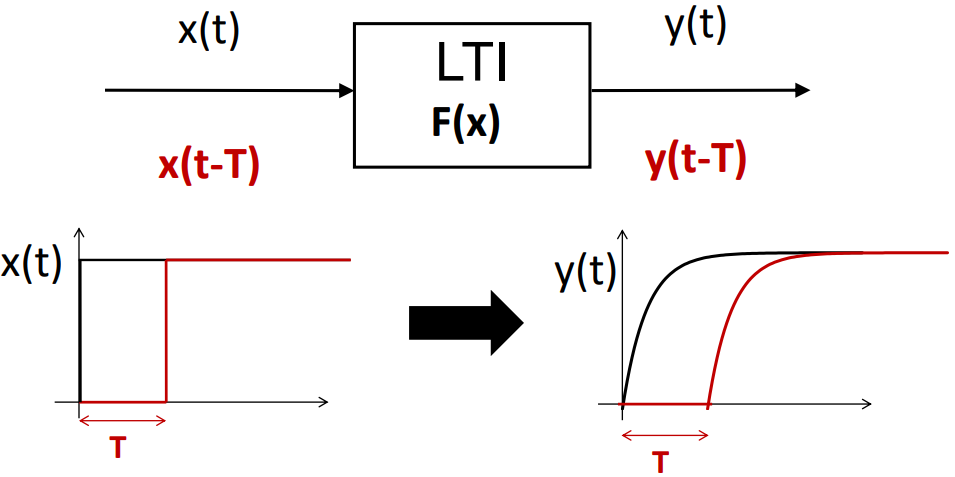
\includegraphics[width = 0.8\textwidth]{../img/blockdiagram8.png}
\end{figure}
\subsection*{Are these models suitable for physical systems?}
These three requirements, whilst simple, are so stringent that \textbf{almost no physical LTI system truly exists}. Consider a car engine - the performance deteriorates over time, to stretch it further, would you expect a system to give the same output after a time delay $T$ of 10 years? Even simple systems such as a resistor in an electrical circuit have non-linearities - a scaling factor $A$ could be chosen for $x(t)$ which would mean too much current flows and the resistor melts.

Most practical systems are not linear, but often we can assume they behave linearly \textbf{under certain conditions/assumptions}. Linear systems are \textbf{much} easier to solve! There are \textbf{analytic} solutions with standard tools used solve the equations. Whereas for non-linear problems it is often necessary to solve them numerically. 
\subsection{Linearisation: Example 1}
For a simple system such as a spring, across all possible compressions or extensions the response is non-linear:
\begin{equation}
  F = -kX
\end{equation}
Hookes law is only a linear approximation of the true response. However, if we choose the operating range of the spring correctly, the response is within the linear region. This approximation is \textbf{valid}.
\subsubsection{Linearisation: Example 2}
Similarly an op-amp has a \textbf{linear region} where the output signals are between supple voltages $V_S$
\begin{figure}[H]
  \centering
  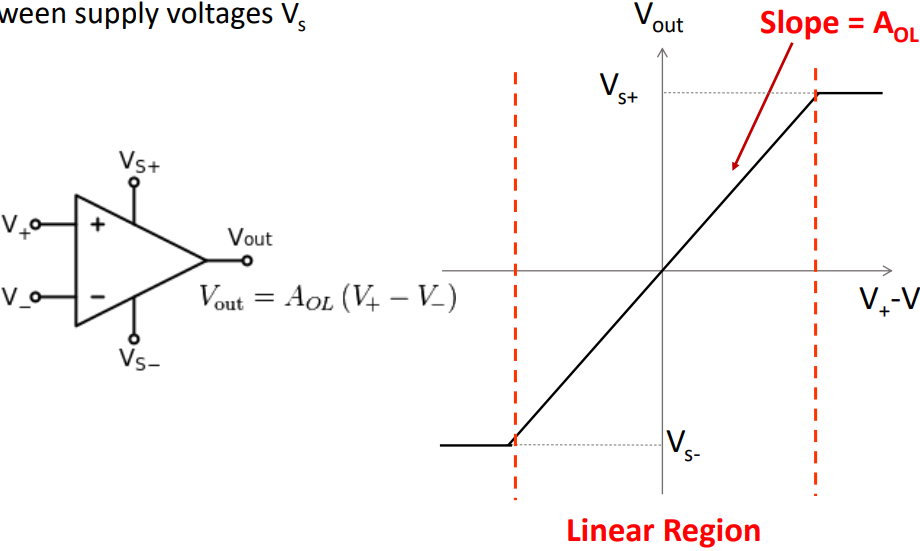
\includegraphics[width = 0.8\textwidth]{../img/graphs4.png}
\end{figure}
Keep signals within these regions and the linear assumption holds:
\begin{figure}[H]
  \centering
  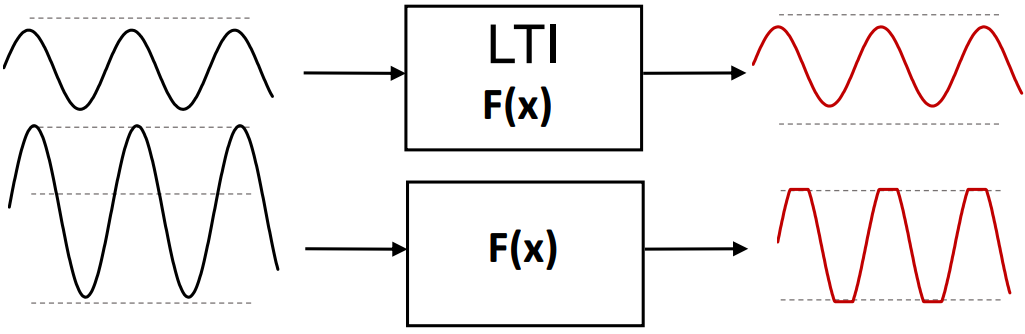
\includegraphics[width = 0.8\textwidth]{../img/blockdiagram9.png}
\end{figure}
Add LTI example
\section{Dynamic systems - Laplace Transform}
\subsection{Dynamic systems as ODEs}
Ideal systems would respond \textbf{instantaneously} to inputs, however real world systems require some time to adjust to changes and are thus known as \textbf{dynamic systems} as the output changes over time.
\begin{figure}[H]
  \centering
  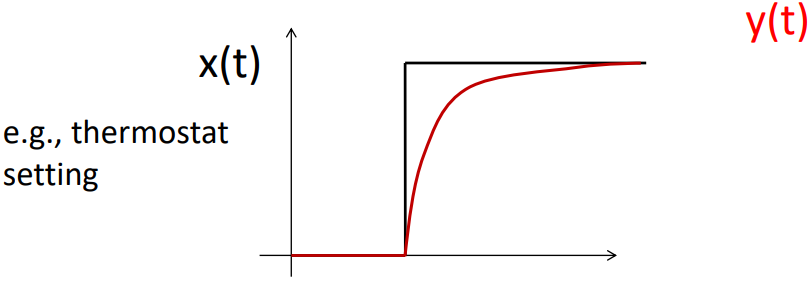
\includegraphics[width = 0.8\textwidth]{../img/graphs5.png}
\end{figure}
As we are intersected in describing something that \textbf{changes} with time, it is useful to express the function block of the system $F(t)$ as an ordinary differential equation (ODE).
\begin{figure}[H]
  \centering
  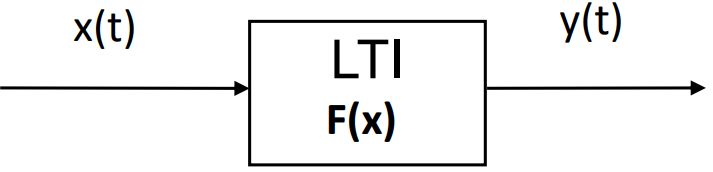
\includegraphics[width = 0.8\textwidth]{../img/blockdiagram10.png}
\end{figure}
\begin{equation}
  \frac{\dif^n y}{\dif t^n} + a_{n-1}\frac{\dif^{n-1}y}{\dif t^{n-1}} + ... + a_2 \frac{\dif^2y}{\dif t^2} + a_1 \frac{\dif y}{\dif t} + a_0 = bx
\end{equation}
\begin{itemize}
  \item $x$ is input function or forcing function
  \item $y$ is output
  \item $n$ is \textbf{order} of the ODE
  \item $a_0...$ are coefficients. These \textbf{completely characterise the system}
\end{itemize}
\subsection{Laplace Transforms}
Because of our \textbf{linear assumptions} we can use Laplace transforms to simplify solving the ODEs. The Laplace transforms of a signal (function) $x$ is the function $X = \Lagr (x)$ defined by
\begin{equation}
  X(s) = \int_{0^-}^\infty x(t) e^{-st} \dif t
\end{equation}
For those $s \in \textbf{C}$ for which the integral makes sense.
\begin{itemize}
  \item $X$ is a complex-valued function of complex numbers
  \item $s$ is called the (complex) \textbf{frequency variable} with units \si{\per\second}, $t$ is called the \textbf{time variable} (in sec); $st$ is unitless
  \item $s = \sigma + j \omega$
\end{itemize}
As we shall see:
\begin{itemize}
  \item Differential operators are replaced with algebraic variables
  \item Algebraic equations are much easier to manipulate \& solve
  \item Standard forms exist for many physical systems
\end{itemize}
\subsubsection{Laplace Transforms: Example 1}
Let's fine Laplace transform $x(t) = e^t$:
\begin{gather}
  X(e^t) = \int_{0^-}^\infty e^t e^{-st} \dif t\\
  X(e^t) = \int_{0^-}^\infty e^{(1-s)t} \dif t\\
  X{e^t} = \left. \frac{1}{1-s}e^{(1-s)t}\right|_{0^-}^\infty \\
  X(e^t) = \frac{1}{1-s} \times 0 - \frac{1}{1-s} \times 1 = \frac{1}{s-1}
\end{gather}
\subsubsection{Laplace Transforms: Example 2}
Constant or \textbf{unit step} $x(t) =1$ (for $t \geq 0$)
\begin{gather}
  X(s) = \int_{0^-}^{\infty} 1 e^{-st}\dif t\\
  X(s) = \int = \left. -\frac{1}{s} e^{-st} \right|_{0^-}^\infty\\
  X(s) = - \frac{1}{s} \times 0 - (- \frac{1}{s}) \times 1 = \frac{1}{s}
\end{gather}
\subsubsection{Laplace Transforms: Example 3}
\textbf{Sinusoid:} first express $x(t) = \cos{(\omega t)}$ as:
\begin{gather}
  x(t) = \frac{1}{2} e^{i \omega t} + \frac{1}{2} e^{-i \omega t} \textrm{ (Euler's formula)}\\
  X(s) = \int_{0^-}^\infty e^{-st} \left( \frac{1}{2} e^{i \omega t} + \frac{1}{2} e^{-i \omega t} \right) \dif t\\
  X(s) = \frac{1}{2} \int_{0^-}^\infty e^{(-s + i \omega)t}\dif t + \frac{1}{2} \int_{0^-}^\infty e^{(-s - i \omega)t} \dif t\\
  X(s) = \frac{1}{2} \frac{1}{s - i \omega} + \frac{1}{2} \frac{1}{s + i \omega} = \frac{s}{s^s + \omega^s} 
\end{gather}
You can look up these transforms in a table. The Laplace variable, s, can be considered to represent the differential operator (very useful for control engineering):
\begin{gather}
  s \equiv \frac{\dif}{\dif t}\\
  \frac{1}{s} \equiv \int_{0^-}^\infty \dif t
\end{gather}
Laplace transform of time derivative $\frac{\dif x}{\dif t}$:
\begin{equation}
  L \left\{ \frac{\dif x}{\dif t} \right\} = \int_{0^-}^\infty \frac{\dif x}{\dif t} e^{-st} \dif t
\end{equation}
Integrating by parts
\begin{equation}
  L \left\{ \frac{\dif x}{\dif t} \right\} = s \int_{0^-}^\infty x(t) e^{-st} \dif t + \left[ x(t)e^{-st} \right]_{0^-}^\infty
\end{equation}
The initial condition $x(0^-)$ is often zero in practice
\begin{equation}
  L \left\{ \frac{\dif x}{\dif t} \right\} = sX(s) - x(0^-) = sX(s)
\end{equation}
We can substitute this result to solve higher order derivatives:
\begin{gather}
  L\left\{ \frac{\dif^2 x}{\dif t^2} \right\} = sL\left\{ \frac{\dif x}{\dif t} \right\} - \frac{dif x}{\dif t} (0^-)\\
  L\left\{ \frac{\dif^2 x}{\dif t^2} \right\} = s^2 X(s) - sx(0^-) - \frac{\dif X}{\dif t} (0^-) = s^2 X(s)
\end{gather}
So more generally, with all initial conditions set to zero:
\begin{equation}
  L\left\{ \frac{d^n x}{dt^n} \right\} = s^n X(s)
\end{equation}
\subsection{Transfer Functions}
After we have taken the Laplace transform of the differential equation of a system, it's useful to rearrange to give the system \textbf{output} as the product of the system \textbf{input} and the system \textbf{transfer function}.
\begin{figure}[H]
  \centering
  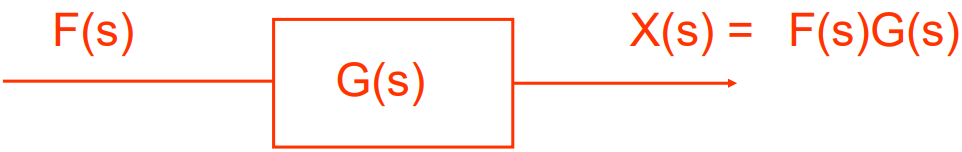
\includegraphics[width = 0.8 \textwidth]{../img/blockdiagram11.png}
\end{figure}
The transfer function of a linear system is defined as the \textbf{ratio} of the Laplace transform of the output variable to the Laplace transform of the input variable, with all the initial conditions assumed to be zero. 
\subsection{Transfer Functions of Mechanical Components}
\subsubsection{Spring}
Convention is input force, output displacement. Balance \textbf{forces}
\begin{figure}[H]
  \centering
  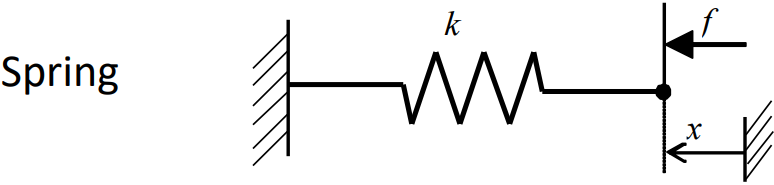
\includegraphics[width = 0.8 \textwidth]{../img/diagram1.png}
\end{figure}
Time domain equation (Hooke's Law): 
\begin{equation}
  f(x) - kx
\end{equation}
$k$ is stiffness in \si{\newton\per\meter}. Laplace domain equation:
\begin{equation}
  F(s) = kX(s)
\end{equation}
Transfer function:
\begin{equation}
  G(s) = \frac{X(s)}{F(s)} = \frac{1}{k}
\end{equation}
\begin{figure}[H]
  \centering
  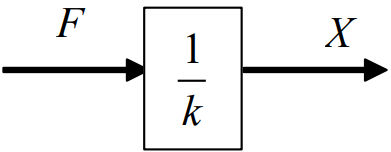
\includegraphics[width = 0.5\textwidth]{../img/blockdiagram12.png}
\end{figure}
\subsubsection{Mass}
Inertial load - mass
\begin{figure}[H]
  \centering
  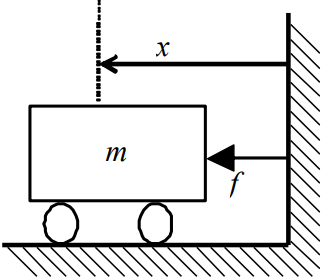
\includegraphics[width = 0.3\textwidth]{../img/diagram2.png}
\end{figure}
Time domain equation from Newton's 2nd law of motion
\begin{equation}
  f(t) = m \frac{\dif^2x(t)}{dt^2}
\end{equation}
Laplace domain equation
\begin{equation}
  F(s) = ms^2 X(s)
\end{equation}
Transfer function
\begin{equation}
  \frac{X(s)}{F(s)} = \frac{1}{ms^2}
\end{equation}
\begin{figure}[H]
  \centering
  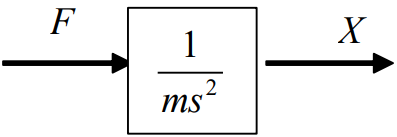
\includegraphics[width = 0.5\textwidth]{../img/blockdiagram13.png}
\end{figure}
\subsubsection{Damper}
Below is a dashpot - a viscous damper. They resist motion through friction. The damping coefficient is in terms of $c$ with units \si{\newton\per\meter\per\second}. Time domain equation:
\begin{equation}
  f(x) = x\frac{\dif x }{\dif t} = csx
\end{equation}
Laplace domain equation:
\begin{equation}
  F(s) = csX(s)
\end{equation}
Transfer function
\begin{equation}
  \frac{X(s)}{F(s)} = \frac{1}{cs}
\end{equation}
\begin{figure}[H]
  \centering
  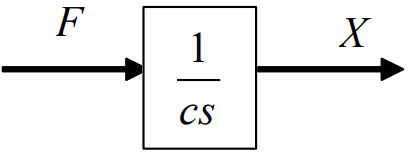
\includegraphics[width = 0.6\textwidth]{../img/blockdiagram14.png}
\end{figure}
\subsection{Combining components}
\subsubsection{Springs}
Springs in parallel
\begin{gather}
  k' - k_1 + k_2\\
  G(s) = \frac{X(s)}{F(s)} = \frac{1}{k'}
\end{gather}
Springs in series
\begin{gather}
  \frac{1}{k'} = \frac{1}{k_1} + \frac{1}{k_2}\\
  G(s) = \frac{X(s)}{F(s)} = \frac{1}{k'}
\end{gather}
\begin{figure}[H]
  \centering
  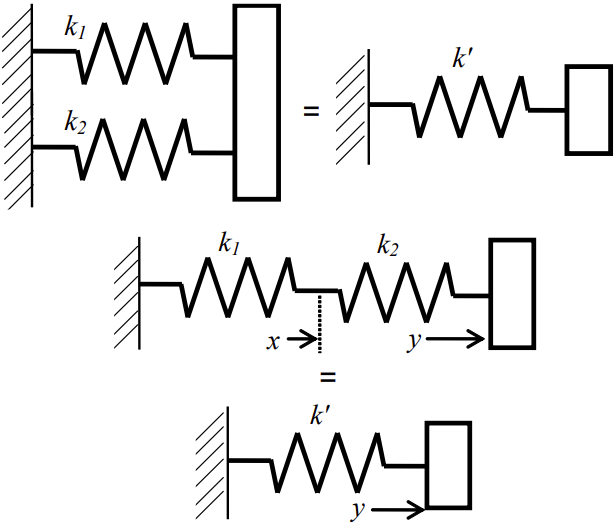
\includegraphics[width = 0.6\textwidth]{../img/diagram4.png}
\end{figure}
\begin{figure}[H]
  \centering
  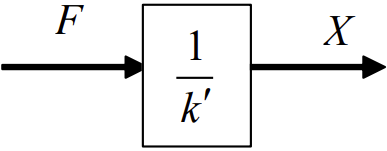
\includegraphics[width = 0.6 \textwidth]{../img/blockdiagram15.png}
\end{figure}
Dashpots behave in a similar way to springs. Parallel:
\begin{equation}
  c' = c_1 + c_2
\end{equation}
and in series:
\begin{equation}
  \frac{1}{c'} = \frac{1}{c_1} + \frac{1}{c_2}
\end{equation}
\subsubsection{Resistor}
Convention is input voltage, output current. Balance voltages.
Ohms law is $V=IR$. Time domain:
\begin{equation}
  v(t) = i(t)R
\end{equation}
Laplace domain:
\begin{equation}
  V(s) = I(s)R
\end{equation}
Transfer function:
\begin{equation}
  G(s) = \frac{I(s)}{V(s)} = \frac{1}{R}
\end{equation}
\begin{figure}[H]
  \centering
  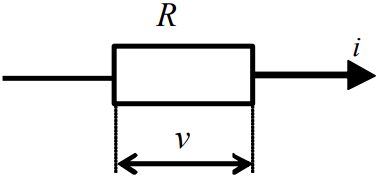
\includegraphics[width = 0.5\textwidth]{../img/diagram5.png}
\end{figure}
\begin{figure}[H]
  \centering
  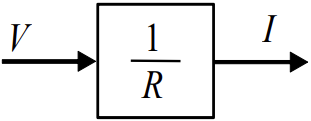
\includegraphics[width = 0.5\textwidth]{../img/blockdiagram16.png}
\end{figure}
\subsubsection{Capacitor}
Either definition of current/voltage relationship gives same result. Time domain:
\begin{gather}
  i(t) = C\frac{\dif v}{\dif t}\\
  v(t) = \frac{1}{C}\int i(t) \dif t
\end{gather}
Laplace domain:
\begin{gather}
  I(s) = CsV(s)\\
  V(s) = \frac{1}{C} \frac{1}{s} I(s)
\end{gather}
Transfer function:
\begin{equation}
  G(s) = \frac{I(s)}{V(s)} = Cs
\end{equation}
\begin{figure}[H]
  \centering
  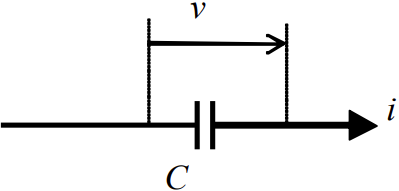
\includegraphics[width = 0.5\textwidth]{../img/diagram6.png}
\end{figure}
\begin{figure}[H]
  \centering
  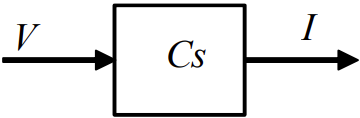
\includegraphics[width = 0.5\textwidth]{../img/blockdiagram17.png}
\end{figure}
\subsubsection{Inductor}
An inductor resists changes of current by generating a voltage in opposition via magnetic induction. From Faraday's Law:
\begin{equation}
  v(t) = L \frac{\dif i}{\dif t}
\end{equation}
Laplace domain
\begin{equation}
  V(s) = LsI(s)
\end{equation}
Transfer function:
\begin{equation}
  G(s) = \frac{I(s)}{V(s)} = \frac{1}{Ls}
\end{equation}
\begin{figure}[H]
  \centering
  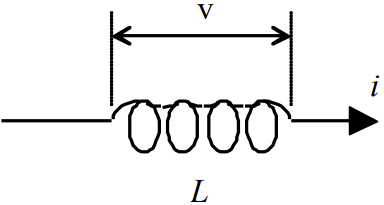
\includegraphics[width = 0.5\textwidth]{../img/diagram7.png}
\end{figure}
\begin{figure}[H]
  \centering
  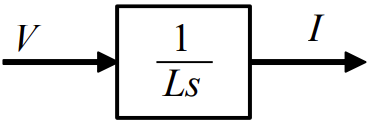
\includegraphics[width = 0.5\textwidth]{../img/blockdiagram18.png}
\end{figure}
\end{document} 